\section{Results}\label{sec3}

Figure \ref{fig:drift_assessment1} illustrates the drift of 16 RFPAs across 10,000 pulses, with RF Length=1.2\,ms, TR=3\,ms, and FA=10\textdegree. Each data point on the graph corresponds to a single RF pulse. The integral of RF magnitude is computed, and the percentage change relative to the initial RF is depicted to visualize the magnitude drift. In this scenario, the highest drift is observed in the case of Tx 16, reaching a value of 23.3\%. The plot reveals the distinction between two distinct groups of RFPA behavior, with one exhibiting less drift than the other. Additionally, the graph indicates that a subset of RFPAs displays fluctuations deviating from the overall trend. Phase drift is determined by calculating the average phase value from the central portion of the RF waveform, which is then subtracted from the phase of the initial RF.

%TC:ignore 
\begin{figure}[h]
    \centering
    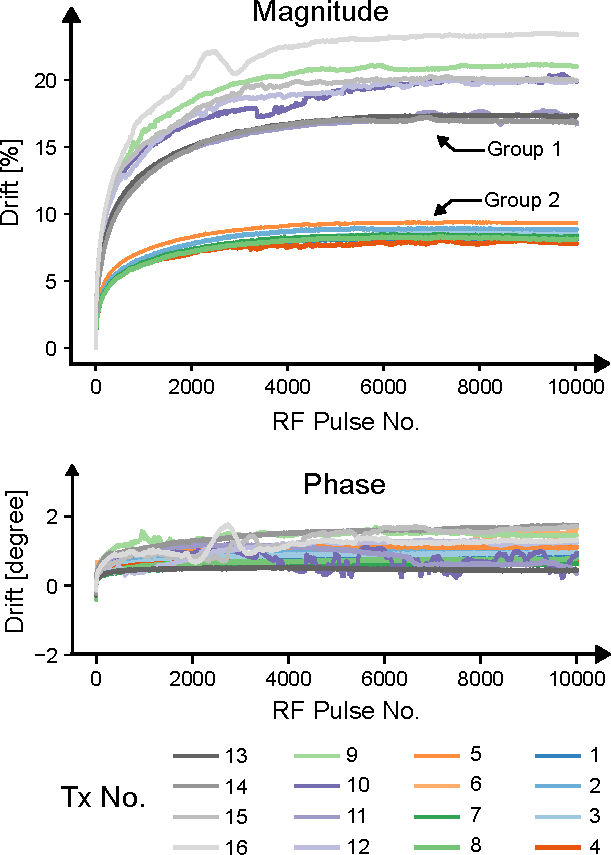
\includegraphics[width=0.5\textwidth]{figures/drift_assesment_plot.pdf}
    \caption{\ Drift of the output of RFPAs during the execution of 10,000 RF pulses with FA of 10\textdegree\, and a duration of 1.2\,ms. TR was set at 3\,ms. Transmit channels 1 to 8 belong to group 2, exhibiting minor drift, while the remaining transmit channels belong to group 1 following the earlier RFPA design. Channel 4 and 16 exhibit the least and greatest magnitude drift, at 7.7\% and 23.3\%, respectively. To quantify magnitude drift, the integral over the magnitude of samples from DICOs records is computed for each pulse, then relative change with respect to the first RF pulse is calculated. Phase drift is determined by calculating the difference between the average phase values extracted from the central portion of DICOs samples in the current RF pulse and initial RF pulse.}
    \label{fig:drift_assessment1}
\end{figure}
%TC:endignore 

Figure \ref{fig:drift_assessment2} displays a synopsis of the inter-pulse RFPA drift evaluation across a range of RF lengths and TR values. Two heatmaps are employed to distinguish the performance of distinct RFPA groups. In this depiction, the color and numerical value denote the average of the maximum drift and the highest drift observed among all RFPAs within the respective group, respectively. It is evident from Figure \ref{fig:drift_assessment2} that there is a correlation between maximum drift and RF duty-cycle. A lengthier RF pulse combined with a shorter TR results in an increased drift within RFPAs. When the ratio of RF length to TR remains constant, the maximum drift consistently falls within a similar range.

%TC:ignore 
\begin{figure*}[t]
    \centering
    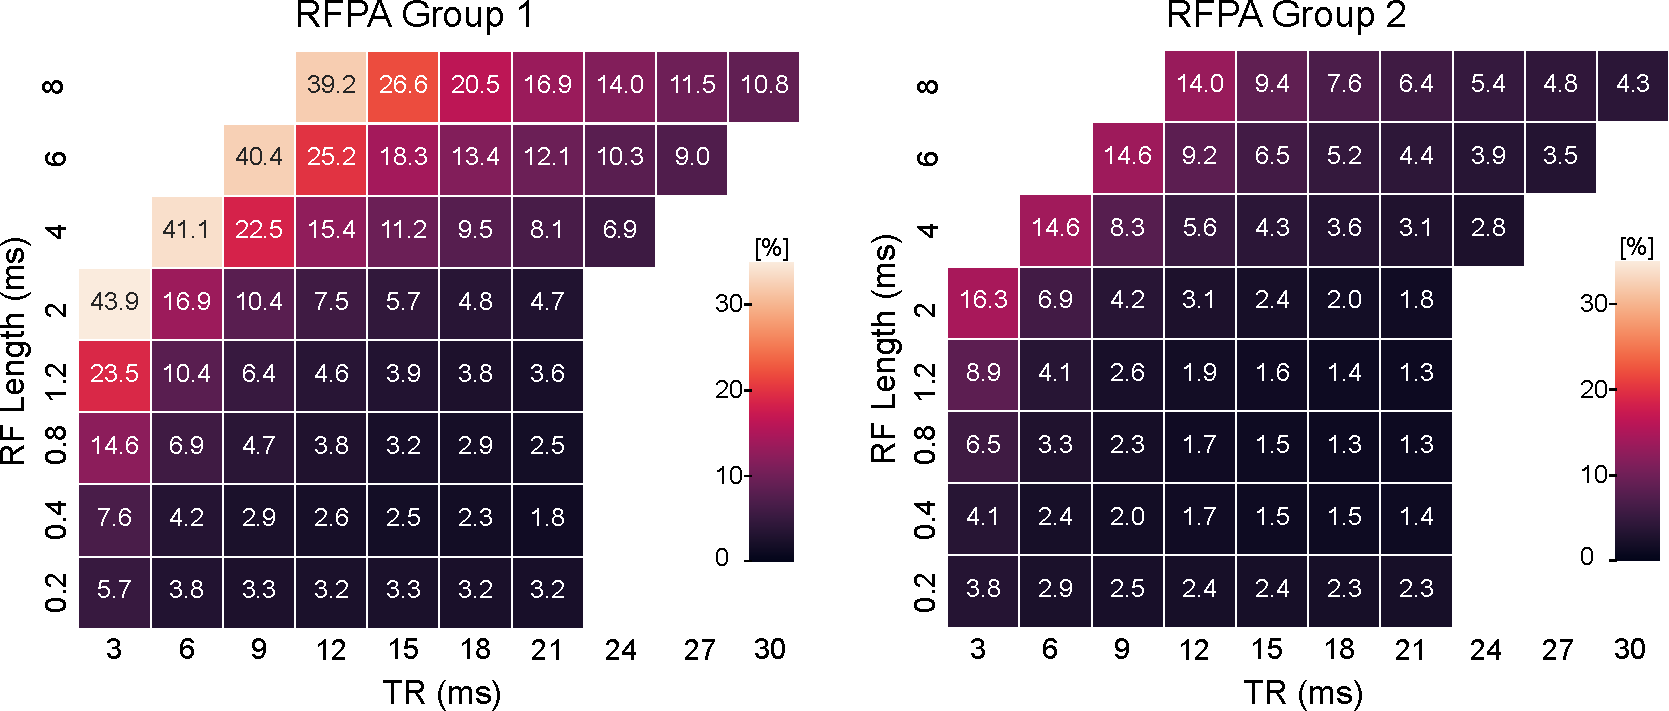
\includegraphics[width=\textwidth]{figures/drift_assesment_table.pdf}
    \caption{\ The inter-pulse drift percentages are presented for various RF lengths and TR. The color and number indicate the average and maximum drift, respectively, for the RFPAs in each group. Each group comprises 8 RFPAs. Notably, RFPAs in group 2 exhibit reduced drift, especially under high RF duty-cycles. The highest RF duty-cycle considered in the examination is 66.6\%. Each block in the heatmap has its own drift plot, as representatively depicted in Figure \ref{fig:drift_assessment1}. }
    \label{fig:drift_assessment2}
\end{figure*}
%TC:endignore 


Figure \ref{fig:drift_assessment3} displays RFPA drift results for different flip angles. The results indicate that when maintaining a constant RF length and repetition time (fixed RF duty-cycle), the impact of the FA on the maximum drift is marginal (corresponding transmit voltages are listed in Table \ref{tab:protocol}). This measurement was conducted using an RF length of 1.2\,ms.

%TC:ignore 
\begin{figure}
    \centering
    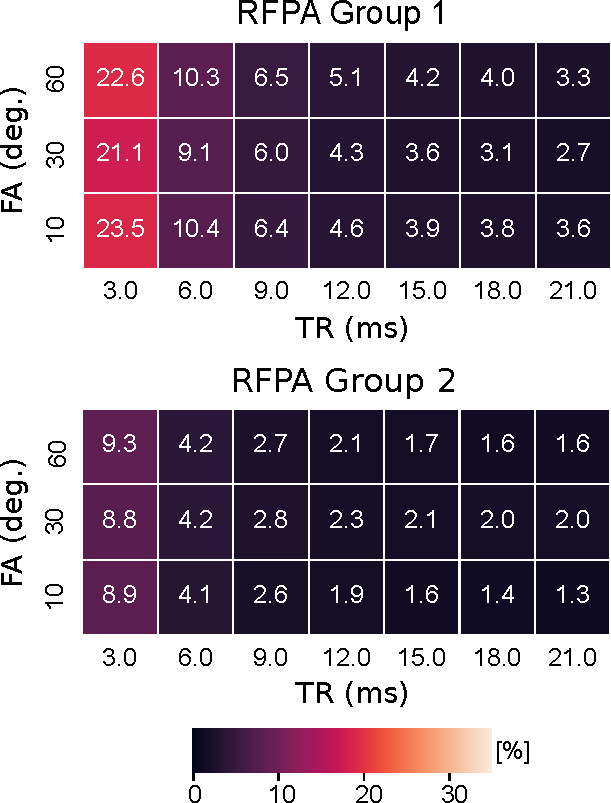
\includegraphics[width=0.4\textwidth]{figures/drift_assesment_table_FA.pdf}
    \caption{\ The dependence of maximum and average drift on FA is assessed across a range of FA and TR, using an RF pulse duration of 1.2\,ms. Within this investigated low transmit voltage range, the impact of FA on drift is found to be negligible.}
    \label{fig:drift_assessment3}
\end{figure}
%TC:endignore 

\marginnote{R1.2}\rev{Figure \ref{fig:inter-scanner} illustrates the plots displaying the drifting of RFPAs obtained from the inter-scanner assessment conducted with an RF length of 1.5\,ms and TR ranging from 3\,ms to 21\,ms. The average drift values in percentage for RFPAs at TR=(3\,ms, 21\,ms) for the involved scanners are as follows: 9.4T group1 and group2 (25.6\%, 2.6\%) and (11.0\%, 1.4\%), 7T Plus (7.9\%, 1.2\%), 7T Terra (10.9\%, 1.2\%), and 11.7T (15.7\%, 2.3\%).} Notably, it is observed that the drift pattern reverses and begins to decrease after reaching its peak at 7T Terra and 11.7T.

%TC:ignore 
\begin{figure*}[t]
    \centering
    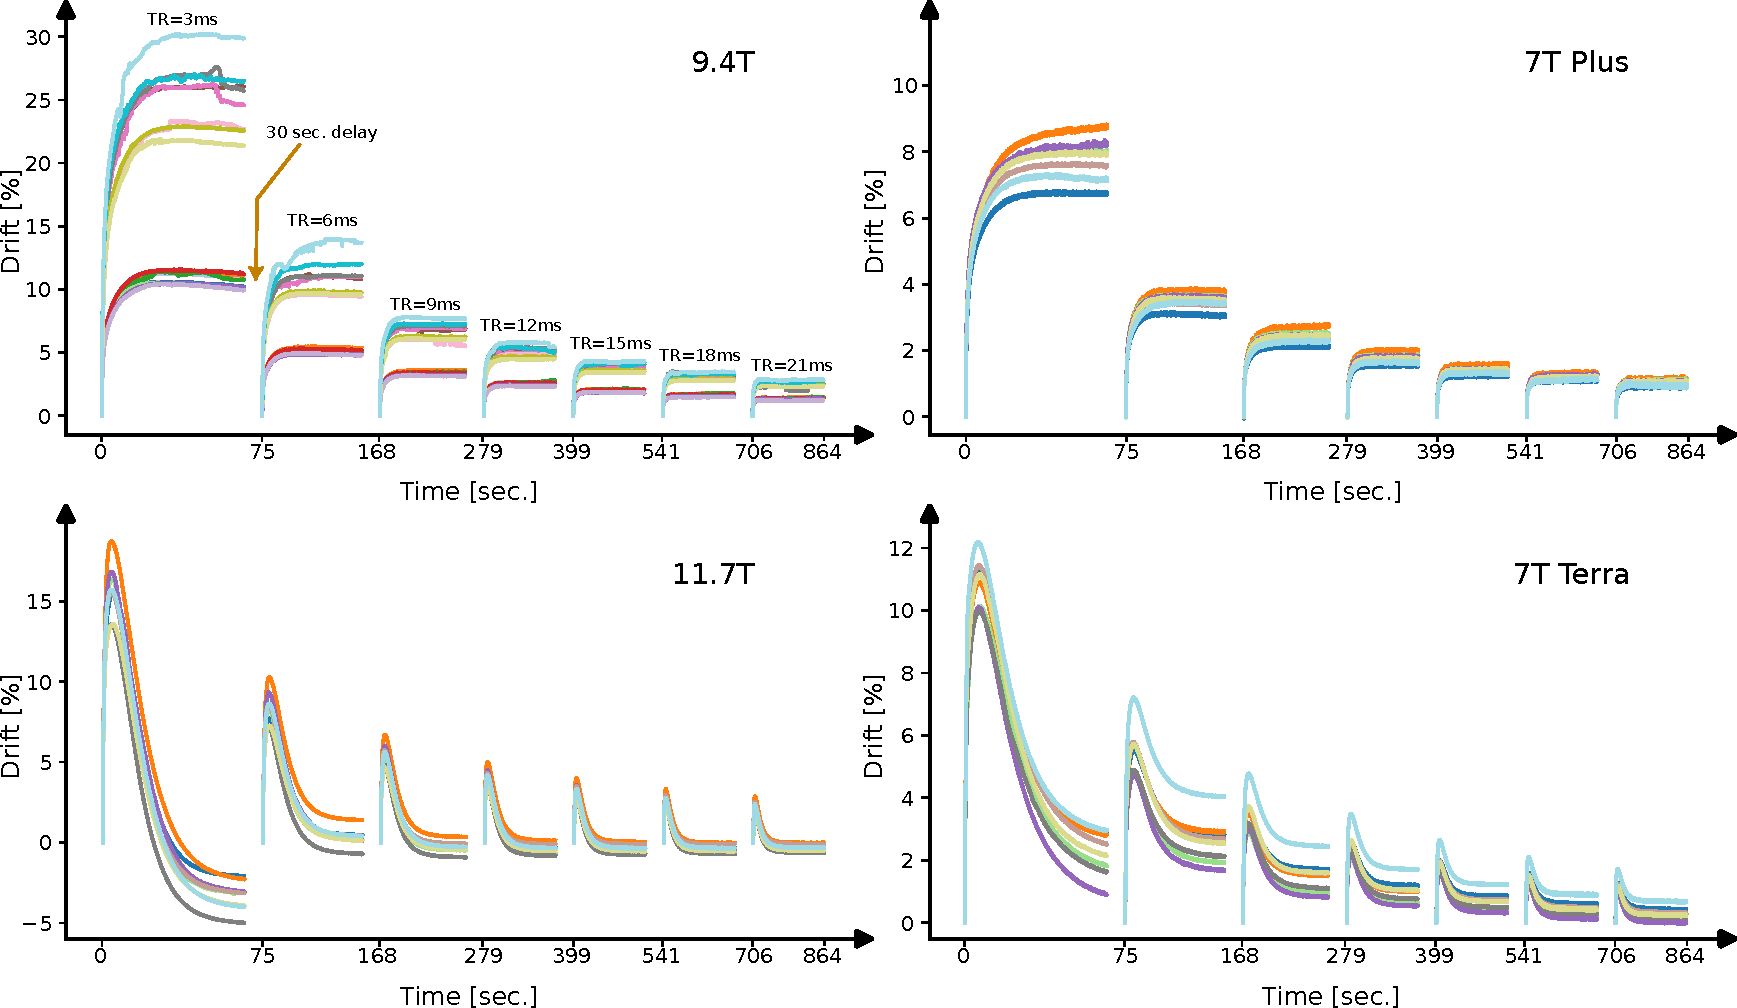
\includegraphics[width=\textwidth]{figures/inter-scanner.pdf}
    \caption{\ The evaluation of intra-pulse drift across four scanners from the same vendor at three distinct field strengths and equipped with RFPAs from the same manufacturer. A rectangular RF pulse of 10\,V lasting 1.5\,ms was played out at certain TR. Measurement was repeated at TRs ranging from 3\,ms to 21\,ms. A 30-second interval was introduced between each repetition to allow the RFPAs to relax. When moving towards repetitions with smaller RF duty-cycles, the number of RF pulses played out decreased due to the anticipated settling of RFPAs after fewer RF pulses. Please note that one of the Tx channels in the 7T Plus plot has been omitted due to malfunction.}
    \label{fig:inter-scanner}
\end{figure*}
%TC:endignore 

Figure \ref{fig:droop} depicts the intra-pulse drift across a range of transmit voltages, averaged over 50 RF pulses each with a duration of 15\,ms. After removing the initial and final 200 samples (equivalent to 200\,us) to eliminate overshoots and undershoots, the magnitude and phase values are normalized to and subtracted from the initial sample, respectively. The plot highlights contrasting RFPA behaviors between low and high transmit voltages. In the case of low transmit voltage, the magnitude drift indicates an increase in RFPA output voltage, while the phase drift remains negligible. Nevertheless, when the transmit voltage exceeds 100\,V per RFPA channel, the RFPA exhibits negative drift, leading to a decline in output voltage, a phenomenon commonly referred to as voltage droop. Furthermore, the phase drift demonstrates more pronounced changes, particularly at very high transmit voltages. Output of transmit channel 1 is depicted in Figure \ref{fig:droop}. Similar behavior is observed in the other transmit channels as well, with the exception that the threshold voltage at which drift direction changes and voltage droop becomes evident is variable and ranges from 100\,V to 125\,V.

%TC:ignore 
\begin{figure*}
    \centering
    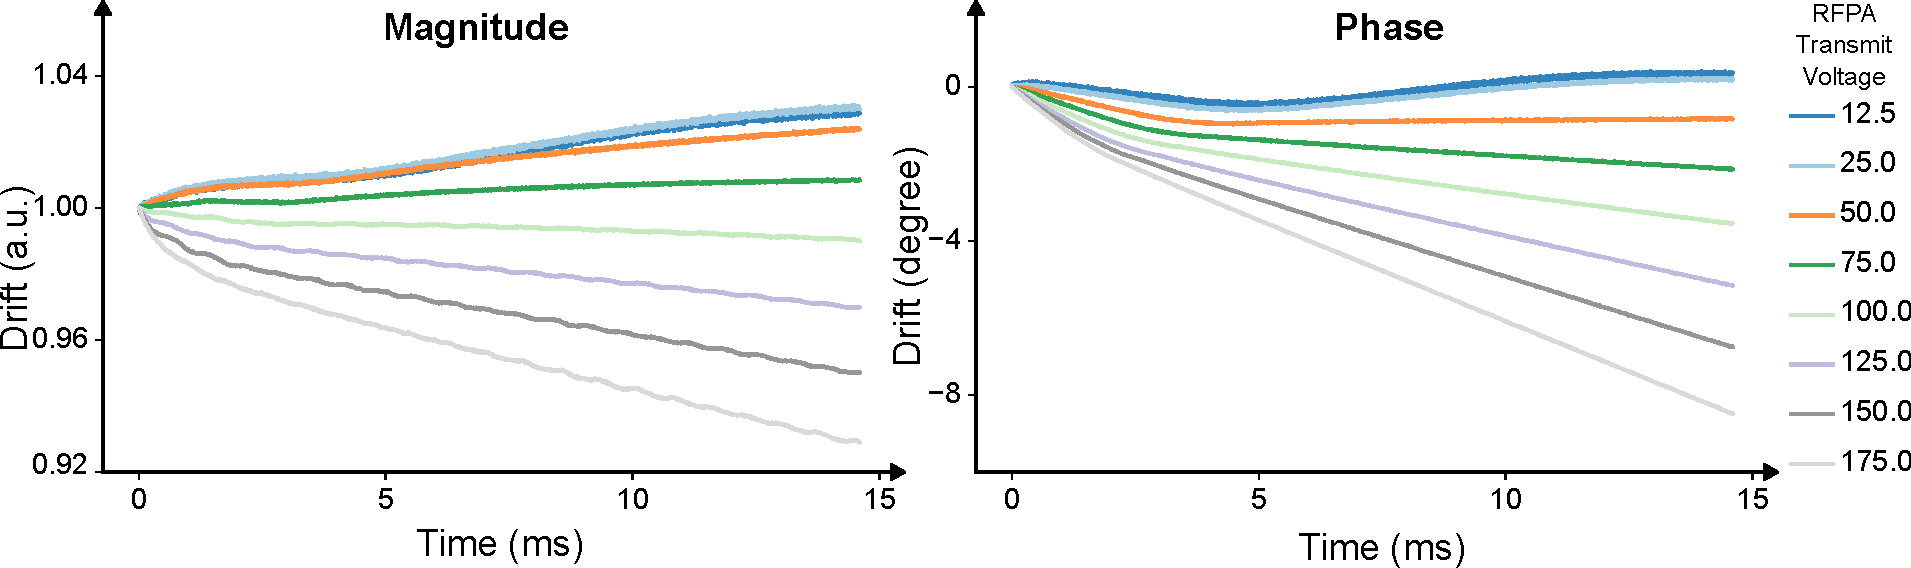
\includegraphics[width=\textwidth]{figures/droop.pdf}
    \caption{\ The intra-pulse drift of transmit channel 1 was assessed by executing a 15\,ms RF pulse across a range of transmit voltages. The RF pulse was repeated 50 times and the DICO samples from these runs were averaged. A 10-second interval between consecutive RF pulses allowed for relaxation of RFPAs. To process the data, the first and last 200 samples were excluded to eliminate overshoots and undershoots. Subsequently, the magnitude of the samples were normalized to the initial sample and the phase of the samples were subtracted from the initial sample. The plot reveals a tendency for intra-pulse drift to rise at low transmit voltages, which gradually diminishes as the transmit voltage increases, until it begins to decline after reaching 100\,V. This loss in output voltage is known as voltage droop. In contrast to low transmit voltages, the phase drift becomes more pronounced at higher transmit voltages.}
    \label{fig:droop}
\end{figure*}
%TC:endignore 

Figure \ref{fig:phantom_drift_result} illustrates the outcomes of bSSFP imaging under three scenarios: without correction, with predictive correction, and with \rev{run}-time correction, all observed with an ascending k-space acquisition order. For comparison, the bSSFP acquisition was repeated with a centric k-space order. The uncorrected results from this experiment are shown in the last row of Figure \ref{fig:phantom_drift_result} (fully corrected results are presented in Supporting Information Figure \ref{sif:bssfp_centric}). In the initial column, unprocessed images from the 40$^\text{th}$ repetition, where steady-state is attained, are displayed. It is noticeable that image intensity is marginally greater when no correction is applied, aligning with simulations indicating that a slight increase in steady-state signal occurs when the target flip angle (FA) of 15\textdegree\, is raised by a small percentage (Supporting Information Figure \ref{sif:bssfp_simulation}). The images contain the signal intensity values for three arbitrarily selected voxels.

The second, third, and fourth columns within Figure \ref{fig:phantom_drift_result} present CV for the initial 10, last 10, and complete repetitions, respectively. \marginnote{R2.7}\rev{CV is computed voxel by voxel within each scan of bSSFP along the repetition dimension. This approach is used to highlight temporal behaviour of RFPA drift which manifests itself along the repetition dimension.} The first repetition is omitted to reduce signal deviations arising from the transient state. The inclusion of RFPA drift corrections in the measurements results in greater temporal consistency which is reflected by lower CV values. It is demonstrated that, in contrast to the scenario without any correction, CV maps exhibit similarity across a range of continuous repetitions in both predictive and \rev{run}-time drift correction methodologies. The outcomes obtained from centric ordering without correction also indicate higher CV compared to its corresponding linear ordering.

The last column in Figure \ref{fig:phantom_drift_result} displays the evolution of voxel intensity across all repetitions for the point marked with a blue cross in the first column. It is observed that voxel intensity increases in presence of RFPA drift for the protocol utilized in this study. In this particular measurement, the RFPAs experience a drift of $10.0\%\pm4.1\%$ (mean $\pm$ SD) in relation to the initial dummy pulse. However, this drift is reduced to $0.64\%\pm0.46\%$ and $0.003\%\pm0.027\%$ through the implementation of predictive and \rev{run}-time correction, respectively.

%TC:ignore 
\begin{figure*}[!htbp]
    \centering
    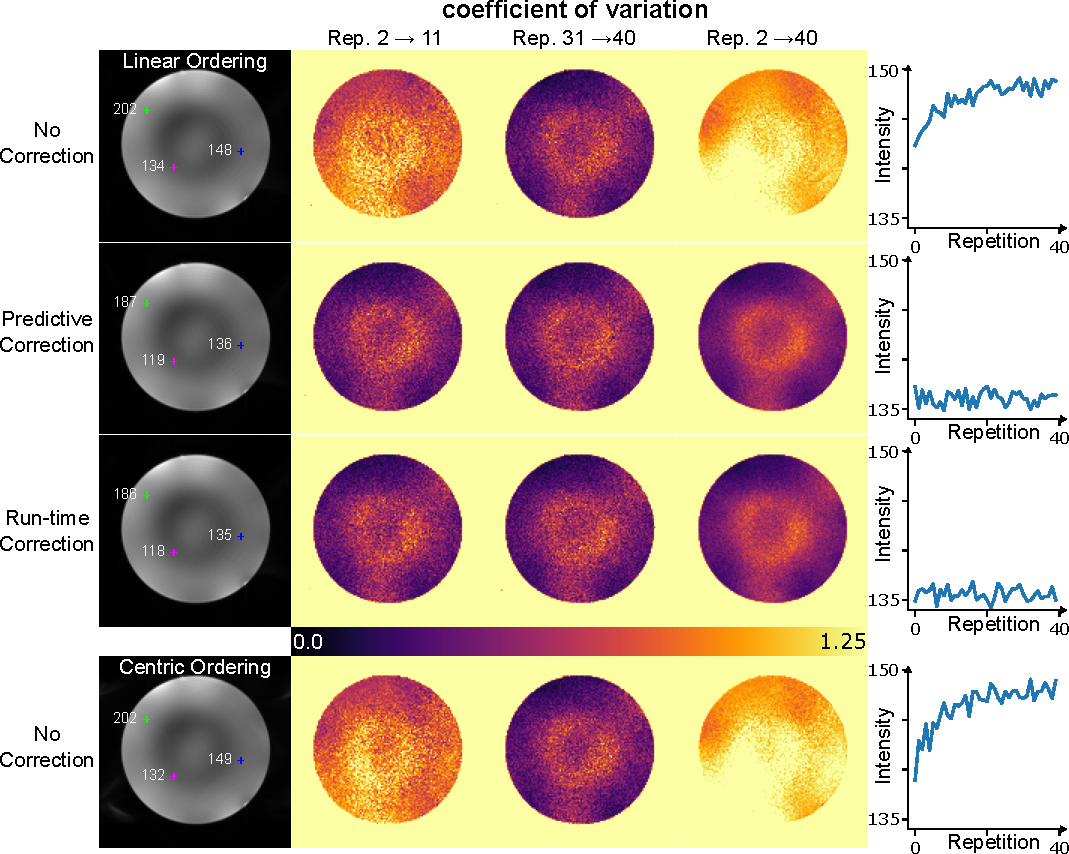
\includegraphics[width=\textwidth]{figures/phantom_drift_result.pdf}
    \caption{\ A comparison between no RFPA drift correction, predictive RFPA drift correction, and \rev{run}-time RFPA drift correction in a phantom study. The initial repetition is excluded from the analysis to mitigate the impact of the transient state. The first column displays reconstructed images from the 40$^\text{th}$ repetition. The intensities of three selected voxels are depicted, revealing higher intensity in the absence of correction. CV is computed across three intervals: the first 10 repetitions, the last 10 repetitions, and all repetitions combined. The application of RFPA correction results in more consistent CV values. The last column showcases the evolution of the voxel marked with a blue cross across all repetitions. Notably, both predictive and \rev{run}-time corrections yield more stable intensity profiles in comparison to the scan without any correction. The final row presents the same scan with a centric ordering scheme, illustrating the greater sensitivity of centric ordering to RFPA drift. }
    \label{fig:phantom_drift_result}
\end{figure*}
%TC:endignore 

 
Figure \ref{fig:sub3_drift_result} illustrates the in-vivo outcomes of RFPA drift correction. Due to the extended $\text{T}_1$ relaxation times of white matter (WM) and gray matter (GM) at 9.4T\cite{zhu2014relaxation}, a lengthier preparation phase is necessary for bSSFP to achieve a steady state. Given that a set of 100 dummy scans are employed in the measurements, data from the initial seven repetitions are omitted in CV calculations to mitigate the impact of the transient state. Columns one, two, and three display the CV values for the first 10, last 10, and entire set of repetitions, respectively. \rev{The last column shows the evolution of average signal intensity within the ROI depicted by blue and green circles} over 40 repetitions in the unprocessed image. The prolonged transient phase is evident in the plots. There is a slight disparity in image intensity between the uncorrected and RFPA drift-corrected results. This finding aligns with the simulation outcome depicted in Supporting Information Figure \ref{sif:bssfp_simulation}. \marginnote{R2.8}\rev{The average signal intensity in both ROIs during the last 10 repetitions is 3.4\% higher when drift correction is disabled compared to the scan utilizing run-time correction.} The results of similar analysis for the second subject are depicted in the Supporting Information Figure \ref{sif:bssfp_subject4}.

%TC:ignore 
\begin{figure*}
    \centering
    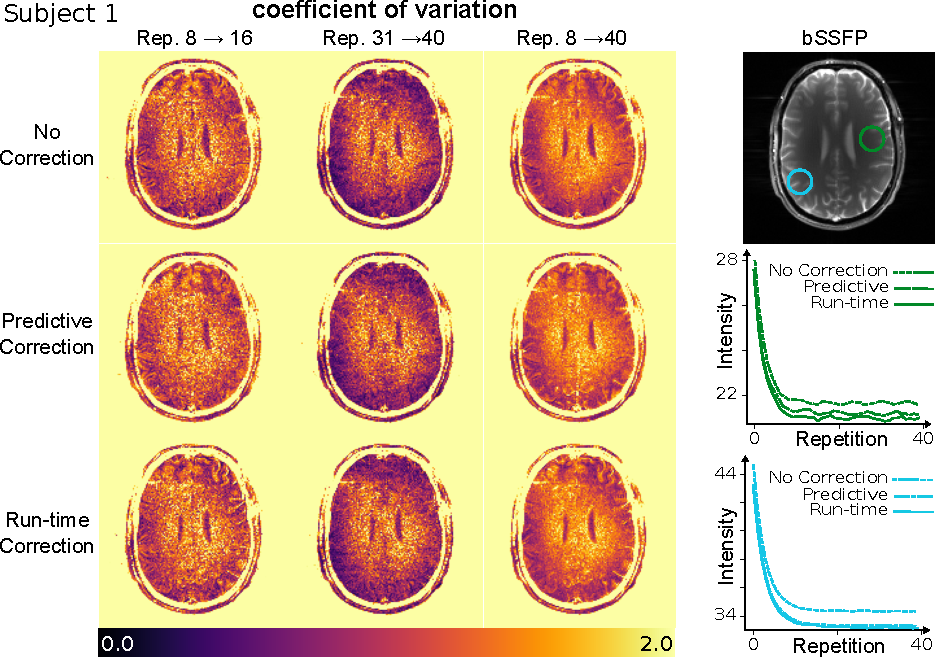
\includegraphics[width=\textwidth]{figures/sub3_drift_result.pdf}
    \caption{\ A comparison through CV calculation is performed between no RFPA drift correction, predictive RFPA drift correction, and \rev{run}-time RFPA drift correction using data from the first subject. The initial seven repetitions out of 40 repetitions are excluded from the analysis to mitigate the impact of the transient state. However, due to the extended $\text{T}_1$ of GM and WM at 9.4T, CV computed in columns one to three is influenced by a combined contribution from both bSSFP transient state and RFPA drift. The difference in CV between RFPA drift corrected and uncorrected cases across the three intervals is minimal. It is evident that the transient state predominates in the first 10 repetitions for all three cases with and without RFPA drift corrections. The final column presents the progression of the mean intensity within the ROI shown with blue and green circles throughout all repetitions. The signal intensity slightly increases when the drift correction is turned off, aligning with the simulation outcomes demonstrated in Supporting Information Figure \ref{sif:bssfp_simulation}.}
    \label{fig:sub3_drift_result}
\end{figure*}
%TC:endignore 


Figure \ref{fig:sub3_drift_plot} depicts the drift observed in RFPAs over the scan shown in Figure \ref{fig:sub3_drift_result}. For clarity, only the drift of four RFPAs is displayed, two from group 1 and two from group 2. Each point on the plot represents the integral over the magnitude of one RF pulse. Averaging over 16 RFPAs, the drift is approximately $10.1\%\pm4.1\%$, which is subsequently mitigated to $0.61\%\pm0.44\%$ and $-0.002\%\pm0.014\%$ through the utilization of predictive and \rev{run}-time correction methods, respectively. Notably, one channel exhibits some deviation from its linear trend in predictive correction approach.

%TC:ignore 
\begin{figure}
    \centering
    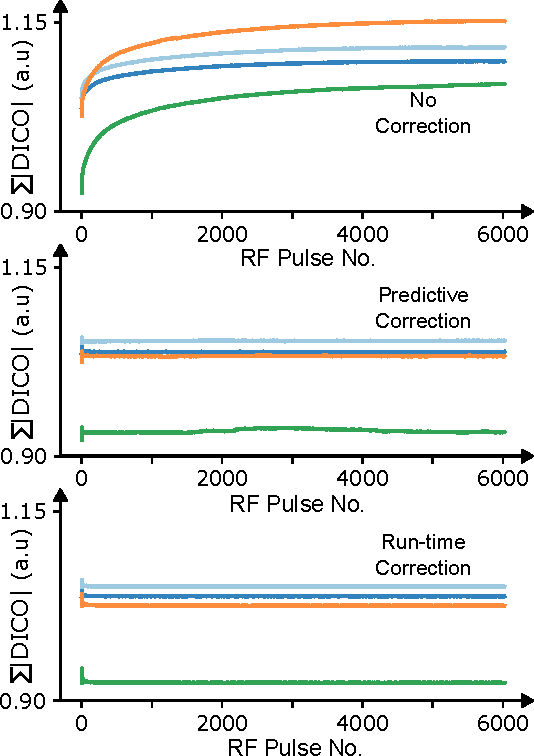
\includegraphics[width=0.4\textwidth]{figures/sub3_drift_plot.pdf}
    \caption{\ The evolution of RFPA drift is depicted for no correction, predictive correction, and \rev{run}-time correction. Ideally, all curves should remain entirely horizontal when there is no drift. Four representative transmit channels (1, 2, 13, and 16) are displayed for clarity. Each point on the plot corresponds to the integral of the magnitude of DICO records.}
    \label{fig:sub3_drift_plot}
\end{figure}
%TC:endignore 


\marginnote{R2.1}\rev{Figure \ref{fig:tflb1} illustrates the comparison of $\mathrm{B_{1}^{+}}$ obtained using the satTFL sequence with RFPA drift correction in both off and on states. First, five sets of $\mathrm{B_{1}^{+}}$ maps are generated from the combination of five consecutive repetition of unsaturated scans along with a presaturated scan. Then, the relative difference between the fifth and fourth $\mathrm{B_{1}^{+}}$ maps and between the fifth and the first $\mathrm{B_{1}^{+}}$ maps is computed for both sets of measurements. It is observed that with drift correction off and on, the relative difference between the fifth and fourth $\mathrm{B_{1}^{+}}$ is minimal because RFPAs are in a steady condition. However, the relative difference between the fifth and the first $\mathrm{B_{1}^{+}}$ is higher when drift correction is off. Conversely, when drift correction is activated, this difference remains minimal again. Within the given slice, approximately 21.4\% and 4.1\% of voxels exhibit a difference larger than 3\% in their $\mathrm{B_{1}^{+}}$ value for the cases of drift correction off and drift correction on, respectively.}


%TC:ignore 
\begin{figure*}
    \centering
    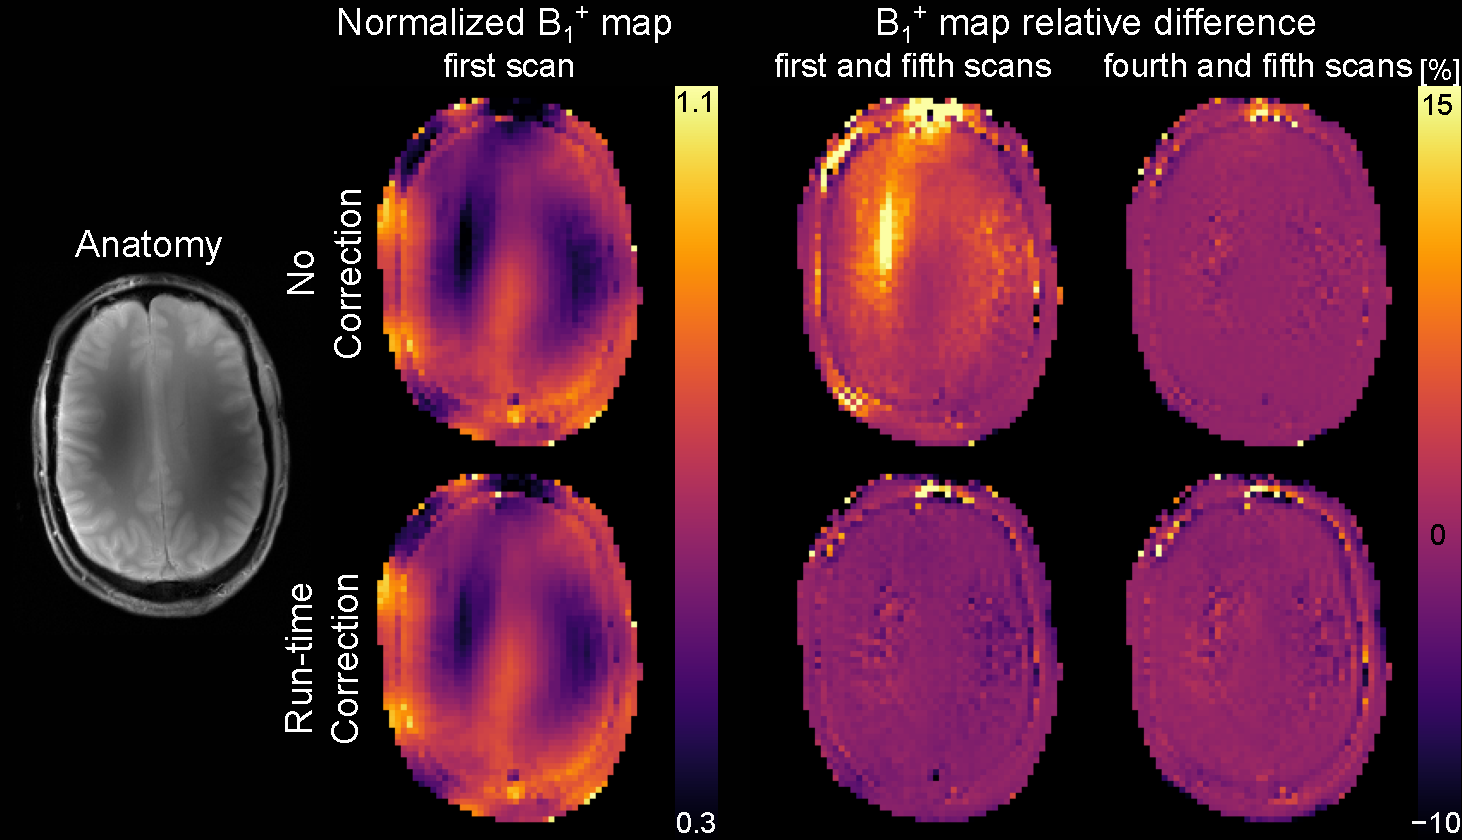
\includegraphics[width=0.8\textwidth]{figures/TFLB1maps.pdf}
    \caption{\ \rev{$\mathrm{B_{1}^{+}}$ reproducibility is evaluated using satTFL sequence while RFPA drift correction turned off and on. Five sets of $\mathrm{B_{1}^{+}}$ maps are generated from five consecutive measurements. Notably, the initial scan is more influenced by RFPA output drift compared to the later scans. Consequently, the relative difference between the $\mathrm{B_{1}^{+}}$ maps calculated from the first and fifth scans is higher than the relative difference between the $\mathrm{B_{1}^{+}}$ maps calculated from the fourth and fifth scans. With RFPA drift correction activated, the temporal drift at the outset becomes acceptably compensated, resulting in a reduction of the relative difference between the first and fifth $\mathrm{B_{1}^{+}}$ maps. $\mathrm{B_{1}^{+}}$ map displayed in the second column is normalized to its nominal value, set at 90\textdegree. }}
    \label{fig:tflb1}
\end{figure*}
%TC:endignore 


% \mycounter{\quickwordcount{05_results}}